
% EDITING GUIDELINES
%
% * Limit lines to no more than 100 characters.  The default should be
%   80 characters.  This leaves room for the addition of 20 new
%   characters on the same line later on.
%
%   RATIONALE: Long lines are hard to read and cause trouble when
%   viewing two versions of the file side by side (e.g., using vimdiff)
%
% * Start every sentence on a new line.
%
%   RATIONALE: This makes sentences so much easier to find using forward
%   search in emacs or vim.
%
% * Do not justify paragraphs.  Particularly, when editing an existing
%   version of the text, do not change line breaks apart from adding
%   line breaks for lines that would otherwise be too long.
%
%   RATIONALE: This makes changes from previous versions so much easier
%   to identify, particularly when using a VCS.  Adding a word and
%   justifying the paragraph may change all the lines in the paragraph,
%   making this look like a huge edit.  Without justification, the
%   diff shows only the addition of the one word.

% ------------------------------------------------------------------------------
\section{Point Location for Triangulations}\label{sec:point_location}
% ------------------------------------------------------------------------------


A common operation in any partition of space is point location, or more
specifically in $\plane$, planar point location.
In Section \ref{sec:applications} we describe a number of queries
that require, as part of the query, identification of the triangle 
containing a point. 
For example, in order to perform a rectangular window query we start by
identifying the triangle containing one of the rectangle's four
corner points.
In this section we describe how to extend our data structure
for triangulations (see Section \ref{sec:tins}), in order to answer point 
location queries efficiently.

Our point location structure is based on that of 
Bose~\etal~\cite{DBLP:journals/talg/BoseCHMM12}.
One important difference between our technique and their's is that we use
a different data structure as the basis for performing point location.
Their construction relies on the point location structure of 
Kirkpatrick~\cite{DBLP:journals/siamcomp/Kirkpatrick83} for which there is no
known external memory version.  
We use the structure of Arge~\etal~\cite{DBLP:conf/alenex/ArgeDT03},
which uses linear space, and answers vertical ray shooting queries in 
$\OhOf{\log_B N}$ I/Os.

We want to design a point location structure which, given a query point $p_q$, 
will return the label of the subregion containing $p_q$. 
Since the subregion fits in internal memory, point location can be carried
out within the sub-region at no additional I/O cost.
We use a two-level search structure.  
The first level allows us to locate the region containing $p_q$, while the 
second allows us to locate the subregion containing $p_q$.
As the  structure is effectively the same at each level, we will only 
describe the structure for locating the region in detail.

Consider the set of region boundary vertices used to partition $\dual{\triang}$. 
These correspond to a subset of the triangles in $\triang$.
We select all the edges of this subset of the triangles of $\triang$,
and insert these into a search structure, which we denote $\N$.
With each edge in $\N$ we associate the label of the region
immediately below it.
If the triangle below an edge is shared by more than one region, as
will often be the case, we can arbitrarily select one. 
Our search structure $\N$ is built using the persistent B-tree structure of 
Arge~\etal~\cite{DBLP:conf/alenex/ArgeDT03} which answers vertical
ray shooting queries.
We repeat this process for each region, creating a search structure
$\N_i$ for each region $\reg[i]$.


In order to determine to which region the query point $p_q$ belongs to we perform a vertical 
ray shooting query from $p_q$ to report the first edge encountered in $\N$
above that point. 
Since we associate with each edge the region below it, the result of this query 
yields the region, $\reg[i]$ containing $p_q$.
We then search in $\N_i$ to locate the sub-region $j$ containing $p_q$.
Finally, we perform an exhaustive search on the triangles of $\subreg[i,j]$
to locate the triangle containing $p_q$.
It is possible, in the event that $p_q \notin \triang$, that the search yields
no result at the cost of searching $\N$, $\N_i$, plus the
the exhaustive search of $\subreg[i,j]$.
This is of course the same cost incurred by a successful search in the worst
case.

There is one important addition yet to make to the search structure $\N$.
Consider the situation depicted in Fig.~\ref{fig:pl_structure}(a), where
we wish to find the triangles containing points $p$ and $q$. 
The ray-shooting query from $p$ correctly returns an edge of the separator
vertically above it; however, the ray starting from $q$ never intersects a 
segment from the separator.

% ------------------------------------------------------------------------------
\begin{figure}
  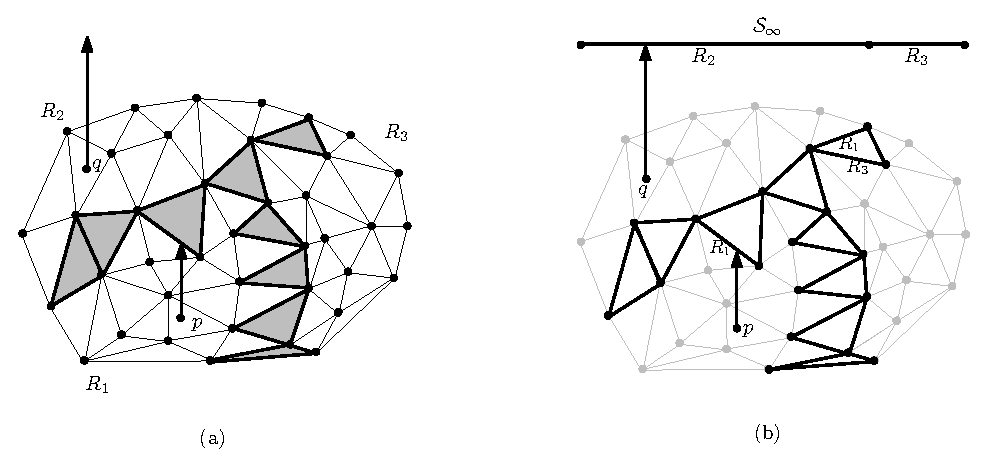
\includegraphics[width=\textwidth]{Fig5}
  \caption[Point location by vertical ray shooting]{In (a), a 
    partitioned triangulation is depicted along with two vertical
    ray shooting queries $p$ and $q$.
    Separator triangles between regions are shaded.
    Recall that the separator is calculated on the dual graph, thus
    the jagged appearance of the separator when drawn in the 
    triangulation.
    Inserting just the edges of boundary triangles into $\N$ is 
    sufficient to handle query $p$ but query $q$ fails.
    In (b), the complete search structure is shown.
    The segments added to $\N$ (drawn as black and heavy) 
    include all boundary triangle edges and the segments generated
    by partitioning $S_{\infty}$.
    Region labels for a small subset of $\N$ are indicated just below
    their respective segments.
    Note that any query falling within $\triang$, and even some outside,
    will return a region to search.
  }
  \label{fig:pl_structure}
\end{figure}
              
In order to ensure that the ray shooting query always reports a valid region, we 
extend our search structure $\N$ as follows.
Let $S_{\infty}$ be a line segment with endpoints at the min and max 
$x$ coordinates of $\triang$, and with $y$ coordinate $+\infty$.
We scan $\triang$ from left to right and split $S_{\infty}$ at any
point where the region immediately below the upper hull changes,
and record for each such segment the region immediately below.
If we insert all the newly-generated segments in $\N$, all vertical ray 
shooting queries within $\triang$ now return a valid result.

\begin{lemma}\label{lem:size_s_infty}
The number of segments added to $\N$ by partitioning $S_{\infty}$
is bounded by the size of the region separator for the subdivision
at the region level. Likewise, the number of segments added 
to all $\N_i$ is bounded by the size of the subregion separators.
\end{lemma}

\begin{proof}
We begin with proving this claim for $\N$.
By definition, $S_{\infty}$ is only split when the region immediately
below the upper hull of $\triang$ changes.
Any such change must occur at a vertex in $\triang$.
Let $v$ be this vertex and an let $t_i$ be a triangle in $\reg[i]$ 
immediately to its left, and $t_j$ a triangle in $\reg[j]$ immediately
to its right, where $t_i$ and $t_j$ are on the upper hull of
$\triang$ (see Fig.~\ref{fig:pl_s_infty}).
Assume for the sake of contradiction that none of the triangles
adjacent to $v$ is a boundary triangle. 
In our construction, no two edge adjacent triangles in $\triang$
can be in different regions unless at least on of them is
a boundary triangle.
Since $t_i$ and $t_j$ are in separate regions if we walk 
from $t_i$ to $t_j$ around $v$, we must arrive at two 
triangles which do not have the same region, since the
region label changes at some point along this walk.
This contradicts the claim that no triangle adjacent to $v$ is 
a boundary triangle.

The proof on the bound for the sizes of each $\N_i$ is 
analogous to that for $\N$.
There is one matter that must be addressed;
the separator algorithm of \cite{Frederickson87} does
not guarantee contiguous regions in $\triang$.
Within a region, this may introduce discontinuities 
that increase the complexity of $S_{\infty}$.
However, the number of such discontinuities is in no case
worse than the size of the region separator over
all $\N_i$. 

\end{proof}

% ----------------------------------------------------------------
\begin{figure}
  \centering
  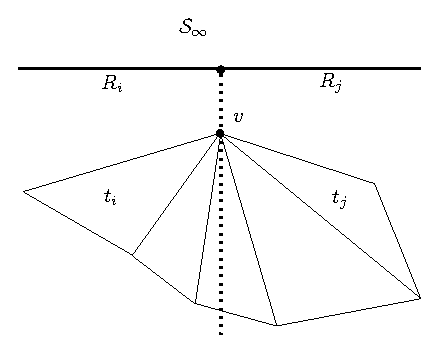
\includegraphics[scale=1.0]{Fig6}
  \caption[Bound on size of $\mathcal{S}_{\infty}$]{
  Illustration of proof that region boundary triangle must
  exists at a break in $\mathcal{S}_{\infty}$.
  }
  \label{fig:pl_s_infty}
\end{figure}
% ----------------------------------------------------------------


\begin{lemma}\label{lem:point_location_space}
By augmenting our terrain data structure with a structure using an additional 
$o(N\bitsPerPoint)$ bits, point location queries can be answered in 
$\OhOf{\log_{\succblksize}{N}}$ I/Os.
\end{lemma}

\begin{proof}
In the top level, region finding, data structure there are 
$\BigOh{ \frac{N}{\sqrt{\succblksize \lg^3 N}} }$ region boundary vertices. 
For each such vertex we insert at most six edges into our search structure;
this includes three edges for each triangle in the separator, plus any edges
added to $S_{\infty}$ by Lemma~\ref{lem:size_s_infty}.
Associated with each edge we must store $2\bitsPerPoint$ bits for the endpoints, 
plus a region label requiring $\lg{ \left( \frac{N}{\succblksize \lg^3 N} \right) }$ 
bits. 
Thus the total space, in bits, required by this structure will be:

\begin{eqnarray}
O\left( \frac{N}{\sqrt{\succblksize \lg^3{N}}} \right) \cdot \left( 2\bitsPerPoint + 
\lg{\left( \frac{N}{\succblksize \lg^3 N} \right)} \right) &=&  
O\left( \frac{N\bitsPerPoint}{\sqrt{\succblksize \lg^3 N}} \right) + 
\OhOf{\frac{N}{\sqrt{\succblksize \lg^3 N}}} \cdot 
\lg{ \left( \frac{N}{\succblksize \lg^3 N} \right) } \nonumber \\
	&=& \ohOf{N\bitsPerPoint} + \ohOf{N} \label{eqn:pl_region_space}
\end{eqnarray}

For the subregion search structures we will consider their space cumulatively.
We add $\OhOf{N/\sqrt{\succblksize}}$ edges, each requiring $2\bitsPerPoint$ bits
for the endpoints,
and $\lg{( \lg^3 N )}$ bit references to the $\lg^3{N}$ sub-regions within the region. 
Again, by Lemma~\ref{lem:size_s_infty}, the addition of edges in $S_{\infty}$ does not 
asymptotically increase the size of the $\N_i$.
The space required for this structure is then:

\begin{equation}\label{eqn:pl_subregion_space}
\BigOh{\frac{N}{\sqrt{\succblksize}}} \cdot ( 2\bitsPerPoint + \lg{(\lg^3{N})} ) = 
\BigOh{ \frac{N\bitsPerPoint}{\sqrt{\succblksize}}} + \BigOh{ \frac{N}{\sqrt{\succblksize}} \cdot \lg{\lg{(N)}}}
\end{equation}

The first term of this equation is clearly $\ohOf{ N \bitsPerPoint }$. 
Recall that $\succblksize = (B \lg N)/(c + \bitsPerPoint)$ and that $B = \OmegaOf{\lg{N}}$. 
Thus, for the second term of Eq.(\ref{eqn:pl_subregion_space}) we have:

\begin{eqnarray}
\BigOh{ \frac{N}{\sqrt{\succblksize}} \cdot 3 \lg{\lg{N}} } &=& 
\BigOh{ \frac{N}{\sqrt{\frac{B \lg N}{c+\bitsPerPoint}}} \cdot \lg{\lg{(N)}} } \nonumber\\
%&\le& \OhOf{ \frac{N\bitsPerPoint}{\sqrt{\lg^2{N}} } \cdot \lg{\lg{N}} } \nonumber\\
&=& \ohOf{N\bitsPerPoint}\label{eqn:pl_subregion_space_final}
\end{eqnarray} 

The total space we use is thus bounded by $\ohOf{ N\bitsPerPoint}$ bits. 
The I/O complexity stems from the fact that we perform two point location 
queries on data structures that answer the query in $\OhOf{\log_B N}$ I/Os.
\end{proof}

\begin{theorem}\label{thm:terrain_with_point_location}
Given a terrain $\triang$, where each point coordinate may be stored in $\bitsPerPoint$ 
bits, there is a data structure that represents $\triang$ in 
$N\bitsPerPoint + O(N) +o(N\bitsPerPoint)$ bits that permits traversal of a path crossing 
$K$ faces in $\triang$ with $O \left( \frac{K}{ \lg{B} } \right)$ I/Os, and which 
supports point location queries with $\OhOf{\log_B{N}}$ I/Os.
\end{theorem} 

\begin{proof}
The terrain data structure requires $N\bitsPerPoint + O(N) +o(N\bitsPerPoint)$ bits by 
Theorem \ref{thm:terrain_traversal}. 
By Lemma \ref{lem:point_location_space}, adding point location requires only 
$\ohOf{N\bitsPerPoint}$ bits, thus the overall space bound is the same and queries 
can be answered in $\OhOf{\log_B{N}}$ I/Os.
\end{proof}
